\chapter{Guidelines and Desiderata for Optimizing the Physical Data Layout and Query Processor in GDBMSs}
\label{c:guidelines}

In this chapter, we review the primary components that form the storage layers of \gls{gdbms}s, \gls{gdbms}'s primary operators and the general data access patterns of operators when evaluating a query. We then draw a basic set of guidelines and desiderata that will instruct the design of the physical data layout and query-processing techniques introduced in later chapters.

Section \ref{sec:property-graph-data-model} briefly describes the \emph{property graph data model}. Section \ref{sec:storage-components} describes the primary storage components of \gls{gdbms}s that adopt the property graph data model, while Section \ref{sec:operators} reviews the query processing operators in \gls{gdbms}s. We end the chapter by stating our guidelines in Section \ref{sec:guidelines}.

\section{Property Graph Data Model}
\label{sec:property-graph-data-model}

\begin{figure}
	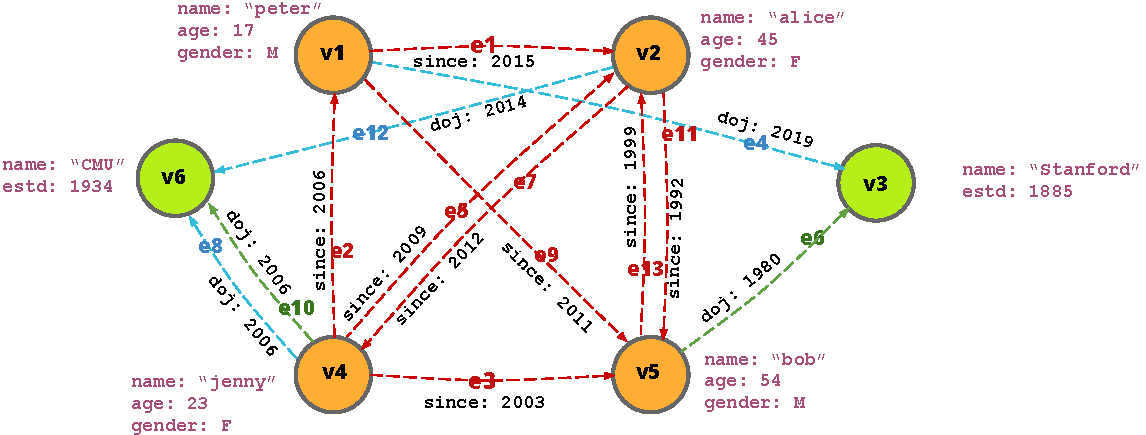
\includegraphics[scale=0.86]{img/property-graph}
	\vspace{-8pt}
	\caption{Running example graph.}
	\label{fig:runn}
	\vspace{-8pt}
\end{figure}

Figure~\ref{fig:runn} shows a graph data, that serves as our running example, in the property graph data model. A property graph consists of \emph{vertices} that represent entities and directed \emph{edges} between vertices that represent relationships between entities. Each vertex and edge has a particular \emph{label}, describing the high-level categories of vertices and edges. For example, in Figure~\ref{fig:runn}, vertices have labels: \texttt{PERSON} and \texttt{ORG}, while edges have labels: \texttt{FOLLOWS}, \texttt{WORKAT} and \texttt{STUDYAT}.

Similar to columns in relational tables, vertices and edges can have (key, value) \emph{properties}. Although the properties of vertices and edges do not need to adhere to a strict \emph{schema}, in practice many of these properties are often highly structured, i.e., a similar set of properties will exist on vertices and edges of the same label.

\section{Primary Storage Components in GDBMSs}
\label{sec:storage-components}

In every \gls{gdbms} we are aware of, the edges of a graph are stored in data structure called \emph{adjacency lists}~\cite{bonifati-adj-lists}. An adjacency list of a vertex $v$ is a list of \emph{adjacent} edges and \emph{neighbouring} vertices of $v$. In a \gls{gdbms}, each vertex has 2 adjacency lists - a \emph{forward adjacency list} containing all outward edges of that vertex, and a \emph{backward adjacency list} that holds all inward edges of the vertex. One can think of edges in the graph as a relational table, having 3 attributes, a source vertex, a destination vertex and an 8-byte edge ID. The adjacency lists can then be thought of as an \emph{index} on this relational table that is \emph{clustered} by either the source or destination vertex. In practice, often this index has a depth of 1 or 2, so given the ID of a vertex $v$, a system can access $v$'s list of edges in a small number of lookups. By having adjacency lists of a vertex in either direction, the system can access the list of outward and inward edges and neighbouring vertices of $u$ in a constant-time lookup operation, which provides the core capability of fast joins on vertices to a \gls{gdbms}. 

Typically, a single-directional adjacency list of vertex $u$ is further clustered into sublists by the edge label of the edges. This enables extending a vertex through its edges with a \emph{particular} label in constant time. The rationale behind the sub-clustering is that many queries by applications have specific labels on query edges. Some systems further order the edge in the adjacency lists either by a property of adjacent edge or neighbour vertex or simply by neighbour vertex's ID. Sorting enables the system to access parts of lists in time logarithmic in the size of the adjacency list.

A \gls{gdbms} also stores properties that appear on the vertices and the edges. There are multiple solutions for storing properties. The most straightforward approach is to store properties in a \emph{key-value store} \cite{dgraph} and use the attribute key and the vertex or edge ID as the key into the store. Properties can also be stored in an interpreted attribute layout \cite{beckmann:sparse}, where a record of a vertex or an edge is a set of attribute-key pairs and is variable-sized. This is better suited than a fixed-size record owing to the randomness of properties over vertex or edge. Searching for a property in variable-sized records involves decoding and parsing the entire record until the matching attribute is found, which can be very slow. Yet another way of storing properties is in a doubly linked-list, as in Neo4j \cite{neo4j}, where the system keeps track of a pointer to the first property record of a vertex or edge and each subsequent property record points to the next. This is not a very optimized storage layout and does not localize and order the properties of vertices and edges. 

\section{Query Execution in GDBMSs}
\label{sec:operators}

In this section, we review the general execution of queries in a \gls{gdbms} by analyzing major operators used in the query plans. Though systems differ in their architectures and implementation of operators that they support for executing queries, there is similarity in their data access patterns. We use the Cypher query language \cite{cypher} to describe the queries we use in our examples. A user query typically consists of 3 parts, 1) a \texttt{MATCH} clause describes a subgraph query pattern $Q(V_Q, E_Q)$, where $V_Q$ and $E_Q$ are the query vertex and edge variables, that the system will match on the input graph; 2) \texttt{WHERE} clause contains a predicate $\rho$ over properties of the edges and vertices that the matched subgraph must satisfy; and 3) a \texttt{RETURN} statement that returns a projection of the variables in the match query or performs a group-by and aggregate information. The \texttt{MATCH}, \texttt{WHERE} and \texttt{RETURN} clauses of a cypher query effectively corresponds to the \texttt{FROM}, \texttt{WHERE} and \texttt{SELECT} clauses of SQL. Example \ref{ex:cypher-example} shows a typical query written in Cypher language, to query the example graph in figure~\ref{fig:runn}.

\begin{example}
	\vspace{19pt}
	\label{ex:cypher-example}
	Consider the following query. 
	{\em 
		\begin{lstlisting}[numbers=none,  showstringspaces=false,belowskip=0pt ]
		MATCH (a:PERSON)$-$[e:WORKAT]$\rightarrow$(b:ORG)
		WHERE a.age $>$ 22 AND b.estd < 2015
		RETURN *\end{lstlisting}
	}
	This query returns all the PERSON vertices and their workplaces, constrained to the condition that the \textsc{\char13}\texttt{age}\textsc{\char13} property of PERSON vertex has a value that is greater than 22 and \textsc{\char13}\texttt{established}\textsc{\char13} property of ORG vertex is less than 2015. a and b are query vertex variables while e is a query edge variable.
\end{example}
\vspace{-5pt}

The following are the major operators used for matching the subgraph pattern and evaluating predicates in a query.

\begin{itemize}
	
	\item \textbf{\texttt{SCAN}}: Scans a set of vertices and edges from the graph topology.
	
	\item \textbf{\texttt{NEIGHBOURHOOD JOIN}}: e.g. \texttt{EXTEND/INTERSECT} in Graphflow; \texttt{EXPAND} in Neo4j. On a high level, the neighbourhood join operator matches the subgraph query pattern $Q$, one edge at a time. Some systems, e.g Graphflow, can match cyclic queries by matching multiple edges at a time. The input to the operator is a partial match, $t$, that has matched $k$ of the query edges of $Q$. For each partially matched $t$, the operator extends $t$ by matching an unmatched query edge $e_q(u_q, v_q)$, where one of $v_q$ or $u_q$ has already been matched in $t$, say $v_q$ has already been matched. The \emph{join} happens by sequentially reading adjacent edges and neighbour vertices from (forward/backward) adjacency list of the matched $v_q$ one or more matched vertices of $t$, to produce a $k+1$-match. The output of the \texttt{JOIN} is the tuple $t$ with $e_q$ and $u_q$ filled.
	
	\item \textbf{\texttt{PROPERTY READER}}: (Vertex/Edge) property reader reads a property value of any vertex or edge that has been assigned to a variable in $V_Q$ or $E_Q$ of a partial match $t$, from the underlying property storage. 
	
	\item \textbf{\texttt{FILTER}}: Given the predicate $\rho$ from the \texttt{WHERE} clause and a partial match $t$ of $Q$, the \texttt{FILTER} operator omits $t$ from the result of the query if $t$ does not pass the predicate $\rho$.
	
\end{itemize}

\begin{figure}
	\hfill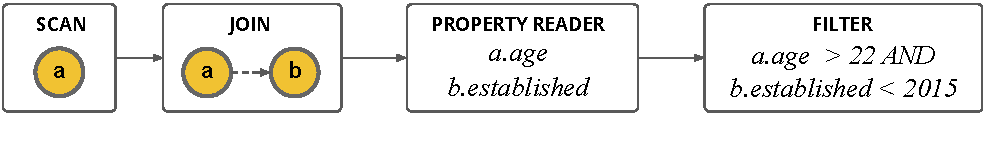
\includegraphics[scale=0.78]{img/ex-qp}\hfill
	\vspace{-10pt}
	\caption{Query plan for Example~\ref{ex:cypher-example}.}
	\vspace{-8pt}
	\label{fig:ex-qp}
\end{figure}

Figure~\ref{fig:ex-qp} shows one of the query plans that the system will generate to execute query in Example~\ref{ex:cypher-example}. It consists of the following sequence of operators: 1) \texttt{SCAN} operator that matches the variable $a$ in query to vertex in the graph having label \texttt{PERSON}; 2) \texttt{PROPERTY READER} reads the property \texttt{age} of the vertex matched to $a$; 3) \texttt{FILTER} operator filter out the partial match based on the contraint $a.age>22$; 4) \texttt{JOIN} operator matches $b$ by reading the forward adjacency list of $a$'s match; 5) \texttt{PROPERTY READER} reads the property \texttt{estd} of $b$'s match; and finally 4) another \texttt{FILTER} operator filters out the matched query pattern that do not confirm to the constraint $b.estd < 2015$.

\section{Guidelines and Desiderata}
\label{sec:guidelines}

We next outline a set of guidelines and desiderata for designing the physical data layout and query processor of a \gls{gdbms}.

\begin{guideline}[Edges are doubly-indexed.]
	\vspace{-5pt}
	Each edge appears in the forward adjacency list of that edge's source vertex and the backward adjacency list of its destination vertex. This results in a 2x replication factor in storing the topology of a graph in the system. This replication cannot be avoided by dropping an adjacency list in any one direction without hampering the capability to perform fast neighbour joins, which is one of the core feature of \gls{gdbms}s. So, we will also doubly index the edges in our design.
\end{guideline}


\begin{guideline}[Edge properties are read in the same order as edges in an adjacency list.]
	\label{ssec:edges-ordered}
	During the execution of a query, the \texttt{JOIN} operator will access the edges of a vertex $v$ in the order these edges appear in $v$'s (forward/backward) adjacency lists. If the query also needs to access the properties of these edges, the access to these edge properties will also be in the same order in which edges were read from the adjacency list. Given that the edges and edge properties are read in order, our first desideratum for the physical data layout and query processor is:
	
	\begin{desideratum}
		Store the properties of edges in the order in which edges are ordered in the adjacency lists and read the edges and their properties sequentially in the operators
	\end{desideratum}
	
\end{guideline}

\begin{guideline}[Vertices cannot be ordered to make access from all neighbour vertices sequential.]
	\label{gdln:vertices-unordered}
	Contrary to how the edges and edge properties can be strictly ordered for each of the adjacency lists, in general, there cannot be ordering on the vertices that completely localizes the access to neighbour vertices of every vertex and the properties of these neighbour vertices without prohibitive data replication. In general, if a vertex $v$ has $n$ neighbours, then $v$ and its properties need to be replicated $n$ times. Hence, localizing access to neighbour vertices and their properties should not be put in the desiderata of the system's physical data layout design.
	
\end{guideline}

\begin{guideline}[Graph data often has partial structure.]
	\label{gdln:graph-schema}
	Even though the property graph data model is semi-structured, in practice many graph databases stored in \gls{gdbms}s have a structure in different components, which \gls{gdbms}s can exploit. One reason this structure exists is that, as observed by prior works \cite{survey}, often the data in \gls{gdbms} comes from structured data in \gls{rdbms}. In fact, several of the \gls{gdbms}s from industry and some academics are actively working on defining a schema language for the property graph data model \cite{schema-validation-bonifati, defining-schema-hartig}. We identify three commonly appearing structure in property graph data:
	
	\begin{enumerate}
		
		\item \textbf{Edge label determines the source and destination vertex labels.} Often, edge labels in the graph data have a well-defined set of source and destination vertex label(s). This restricts the vertices to having inward or outward edges of only a definite set of labels. In our example graph, edges with label FOLLOWS only exists between vertices of label PERSON.
		
		\item \textbf{Edge label has fixed cardinality.} The number of edges of a particular label to which a source or destination vertex can be associated is a property of the edge label. We call this the \emph{cardinality} of an edge label. \emph{One-to-one} cardinality for a label $l_e$ means that each source vertex can be connected to at most one destination vertex through an edge with label $l_e$ and vice versa. \emph{Many-to-one} permits a single edge of a label from a source vertex but multiple edges to a destination vertex. Similar analogy can be applied to \emph{one-to-many} and \emph{many-to-many} cardinality edge labels.
		
		\item \textbf{Label determines properties on vertices and edges.} Similar to the attributes of a relational table, properties on an edge or vertex and the datatypes of these properties can \emph{often} be determined by its edge or vertex label. In our example graph, all vertices having label PERSON have 3 properties: name: \texttt{STRING}, age: \texttt{INT} and gender: \texttt{STRING}. As long as a significant fraction of vertices and edges with a particular label have a common set of properties, a system can exploit this structured to store these properties more efficiently. 
		
	\end{enumerate}
	
	Such structure in data provides an opportunity to design more efficient and simpler data structures for accessing the storage layer of \gls{gdbms}. Our second desideratum is:
	
	\begin{desideratum}
		Exploit the above three commonly appearing structure in the graph data to, 1) compress the data to save space, and 2) provide faster access to the data.
	\end{desideratum}
	
	However, not all data in graph databases have structure. As a working terminology, we will use the following terms:
	
	
	\begin{itemize}
		\item \textbf{Structured/unstructured edge:} An edge of a particular label, that follows above-mentioned points \ref{gdln:graph-schema-rule1} and \ref{gdln:graph-schema-rule2}, is called an structured edge. An edge that is not structured, is called an unstructured edge.
		
		\item \textbf{Structured/unstructured property:} A structured property is a property on a vertex or edge that, 1) can be determined by the vertex type or edge label of that entity; 2) appears in a significant fraction of the vertices of edges of a particular label; and 3) have the same data type in all its occurrence. Any property that is not a structured property, is considered unstructured.
		
	\end{itemize}
	
	
	We focus on optimizing the storage of structured part of the graph data in this thesis. It forms an interesting research topic to optimize a system for unstructured part of graph data. A standard approach is to serialize the key, datatype and value of each property in variable-length records. Structured property storage can, however, be optimized to benefit memory footprint as well as access performance.
	
\end{guideline}

\begin{guideline}[Queries read a small subset of the vertex or edge properties]
	In order to understand the nature of queries user ask on \gls{gdbms}, we conducted a survey of 100 StackOverflow questions containing openCypher queries. We focused on queries of analytical nature and discarded transactional ones like insert, delete and update. We observe the following: 
	
	
	\begin{itemize}
		
		\item Out of the 100 queries, 68 accessed at least one of the properties on a vertex or an edge. Of these, 61 accessed vertex properties and 13 accessed edge properties.
		
		\item Only 11 queries returned all the properties of a query edge or vertex, while 35 of them return specific properties.
		
		\item Average number of properties accessed by those queries that explicitly return a set of properties was only 1.6.
		
	\end{itemize}
	
	We can observe that vertex properties are more popularly accessed as compared to edge properties and most of the queries only access 1 or at most 2 properties. This observation leads to our third desideratum:
	
	\begin{desideratum}
		Allow fast access to individual properties of multiple vertices instead of all properties of a single vertex.
	\end{desideratum}
	
\end{guideline}
